\documentclass{beamer}
\usetheme{Boadilla}
\usecolortheme{default}
\usepackage{amssymb} %maths
\usepackage{amsmath} %maths
\usepackage[utf8]{inputenc} %useful to type directly diacritic characters
\usepackage[T1]{fontenc}

\usepackage{empheq} % for fancy equation boxes
\usepackage{tikz}

\usepackage[polish]{babel}
\usepackage{polski}


\newcommand{\p}{\mathbb{P}}
\newcommand{\E}{\mathbb{E}}
\newcommand{\N}{\mathbb{N}}
\newcommand{\R}{\mathbb{R}}
\newcommand{\1}{\mathbb{1}}

\newcommand{\T}{\mathcal{T}}
\newcommand{\F}{\mathcal{F}}

\newcommand{\Time}{\mathfrak{T}}
\newcommand{\Lap}[1]{\overset{\sim}{#1}}



% <<<<<<<<<<<<<<<<<<<<<<<<<<<<<<<<<<<<<<<<<<<<<<<<<<<<<<<<<<<<<<
%%% No idea emoti

\newcommand{\shrug}[1][]{%
\begin{tikzpicture}[baseline,x=0.8\ht\strutbox,y=0.8\ht\strutbox,line width=0.125ex,#1]
\def\arm{(-2.5,0.95) to (-2,0.95) (-1.9,1) to (-1.5,0) (-1.35,0) to (-0.8,0)};
\draw \arm;
\draw[xscale=-1] \arm;
\def\headpart{(0.6,0) arc[start angle=-40, end angle=40,x radius=0.6,y radius=0.8]};
\draw \headpart;
\draw[xscale=-1] \headpart;
\def\eye{(-0.075,0.15) .. controls (0.02,0) .. (0.075,-0.15)};
\draw[shift={(-0.3,0.8)}] \eye;
\draw[shift={(0,0.85)}] \eye;
% draw mouth
\draw (-0.1,0.2) to [out=15,in=-100] (0.4,0.95); 
\end{tikzpicture}}
% <<<<<<<<<<<<<<<<<<<<<<<<<<<<<<<<<<<<<<<<<<<<<<<<<<<<<<<<<<<<<

\graphicspath{ {./graphics/} }

\title{Resetowanie Stochastyczne}
\subtitle{OMatKo 2023}
\author{Bartosz \.Zbik}
\institute{UJ, Kraków}
\date{1-3 grudnia 2023}







\begin{document}

\begin{frame}
\titlepage
\end{frame}

\begin{frame}
\frametitle{Plan wystąpienia}
\tableofcontents
\end{frame}



\begin{frame}
\frametitle{Pojęcia wstępne, notacja}
Zmienne losowe definiuję na przestrzeni probabilistycznej $(\Omega, \F, \p)$. \\~\\

Zmienna losowa $X$, to intuicyjnie obiekt, który zachowuje się jak rzut kością (jest losowy).\\~\\

Wartość oczekiwaną ze zmiennej losowej $X$ oznaczam $\E X$. Intuicyjnie jest to średnia z $X$.\\~\\

Proces stochastyczny $(X_t)_{t \in \Time}$, to rodzina zmiennych losowych indeksowanych czasem $t \in \Time$. \\~\\

Różne znaczenia liter t, T i $\tau$ (bo innych liter nie ma): \\
 $t$ - czas, $T$ - zmienna losowa, $\tau$ - FPT, $\T$ - MFPT i $\Time$ - zbiór czasu.

\end{frame}

\section{Proces Wienera}
\begin{frame}
\frametitle{Proces Wienera (ruchy Browna) - definicja}
\begin{block}{Definicja}
Proces $W = (W_t)_{t \in [0, \infty)}$ nazywamy procesem Wienera jeśli:
\begin{itemize}
\item $W_0 = 0, ~\p$ - p.n.
\item $W$ ma przyrosty stacjonarne i niezależne
\item $W$ ma ciągłe trajektorie
\item $W_t - W_s \sim \mathcal{N}(0, t-s)$
\end{itemize}
\end{block}
\begin{block}{Intuicja}
Proces Wienera $W = (W_t)_{t \in [0, \infty)}$, to błądzenie przypadkowe w czasie ciągłym.
\end{block}

Dla wygody będziemy czasem zakładać, że $W_0 = x_0, ~\p$ - p.n.
\end{frame}

\begin{frame}
\frametitle{Proces Wienera - trajektorie}
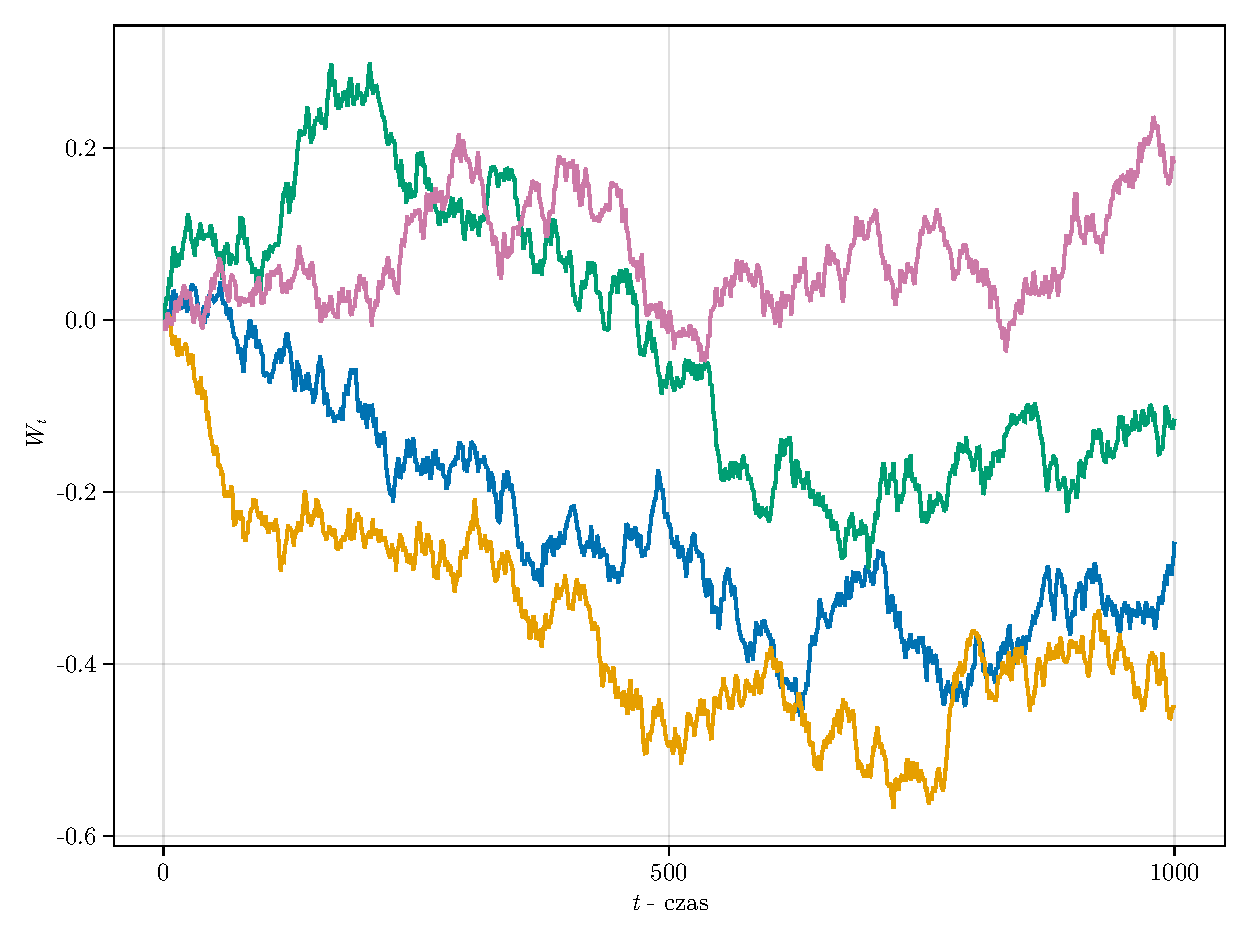
\includegraphics[width=0.9\textwidth]{wiener-sim/only-tr.pdf}
\end{frame}

\section{Problem pierwszej ucieczki}

\begin{frame}
\frametitle{Problem pierwszej ucieczki (ang. first passage time) FPT}
\begin{block}{Definicja}
Niech $(X_t)_{t \in \Time}$ - proces stochastyczny, $A$ - podzbiór $\R$. Zmienną losową $\tau: \Omega \to \Time$ nazwiemy czasem pierwszej ucieczki z $A$ (w skrócie FPT) jeśli
\begin{equation}
\tau = \inf{\{ t : t \in \Time~,~ X_t \notin A \}}.
\end{equation}
Jeśli dla pewnego $\omega \in \Omega$  mamy $\forall t \in \Time: X_t(\omega) \in A$, to kładziemy $\tau(\omega) = +\infty$.
\end{block}

\begin{block}{Intuicja}
Czasem pierwszej ucieczki (FPT) nazywamy zmienną losową, która odpowiada chwili w czasie, w której proces po raz pierwszy uciekł z przedziału (ogólniej zbioru).
\end{block}
\end{frame}


\begin{frame}
\frametitle{Proces Wienera - ucieczka z przedziału (-0.6, 0.1)}
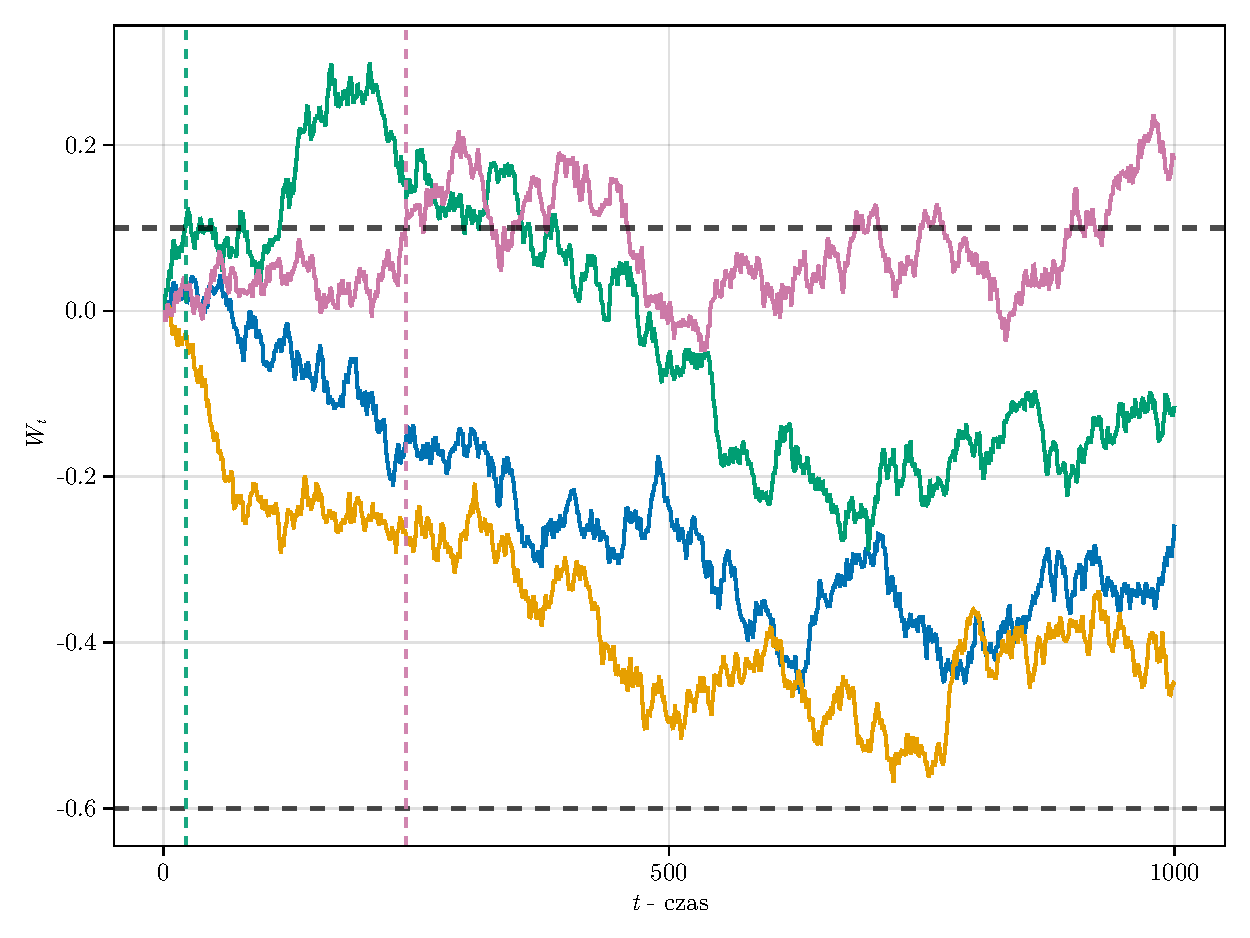
\includegraphics[width=0.9\textwidth]{wiener-sim/tr-with-bounds.pdf}
\end{frame}

\begin{frame}
\frametitle{Po co to wszystko?}
W różnych zastosowaniach praktycznych interesuje nas \\ \emph{średni czas ucieczki}~$\T$ (ang. mean first passage time) 
\begin{equation}
\T := \E \tau~.
\end{equation}
Skrótowo będziemy pisali MFPT. \\~\\

\pause
Postawmy pytanie: \emph{Jak zminimalizować ten czas?} \\~\\
\pause
Możliwe rozwiązanie: \textbackslash title

\end{frame}





\section{Resetowanie}

\begin{frame}
\frametitle{Resetowanie Stochastyczne - resetowanie procesu}
Załóżmy, że mamy proces $(X_t)_{t \in \Time}$, który startuje w $x_0$ (czyli $X_0 \equiv x_0$).\\
Niech $R:\Omega \to \Time$ będzie niezależne od $(X_t)_{t \in \Time}$.
\begin{block}{Definicja (nieformalna)}
Zdefiniujmy\footnotemark{} $(X^r_t)_{t \in \Time}$ ("proces resetowany") jako
\begin{equation}
X^r_t = \begin{cases}
X_t &,~\text{gdy}~ t < R \\
Y_{t-R}^r &,~\text{gdy}~ t \ge R~,
\end{cases}
\end{equation}
gdzie $(Y_t^r)_{t \in \Time}$ jest niezależną kopią procesu resetowanego $(X_t^r)_{t \in \Time}$.
\end{block}

\footnotetext{Bardziej formalnie można użyć ciągu i.i.d. zmiennych losowych o rozkładach jak $R$\\
 i ciągu procesów o rozkładach jak $(X_t)_{t \in \Time}$.}
\end{frame}

\begin{frame}
\frametitle{Resetowanie procesu - przykład dla procesu Wienera}
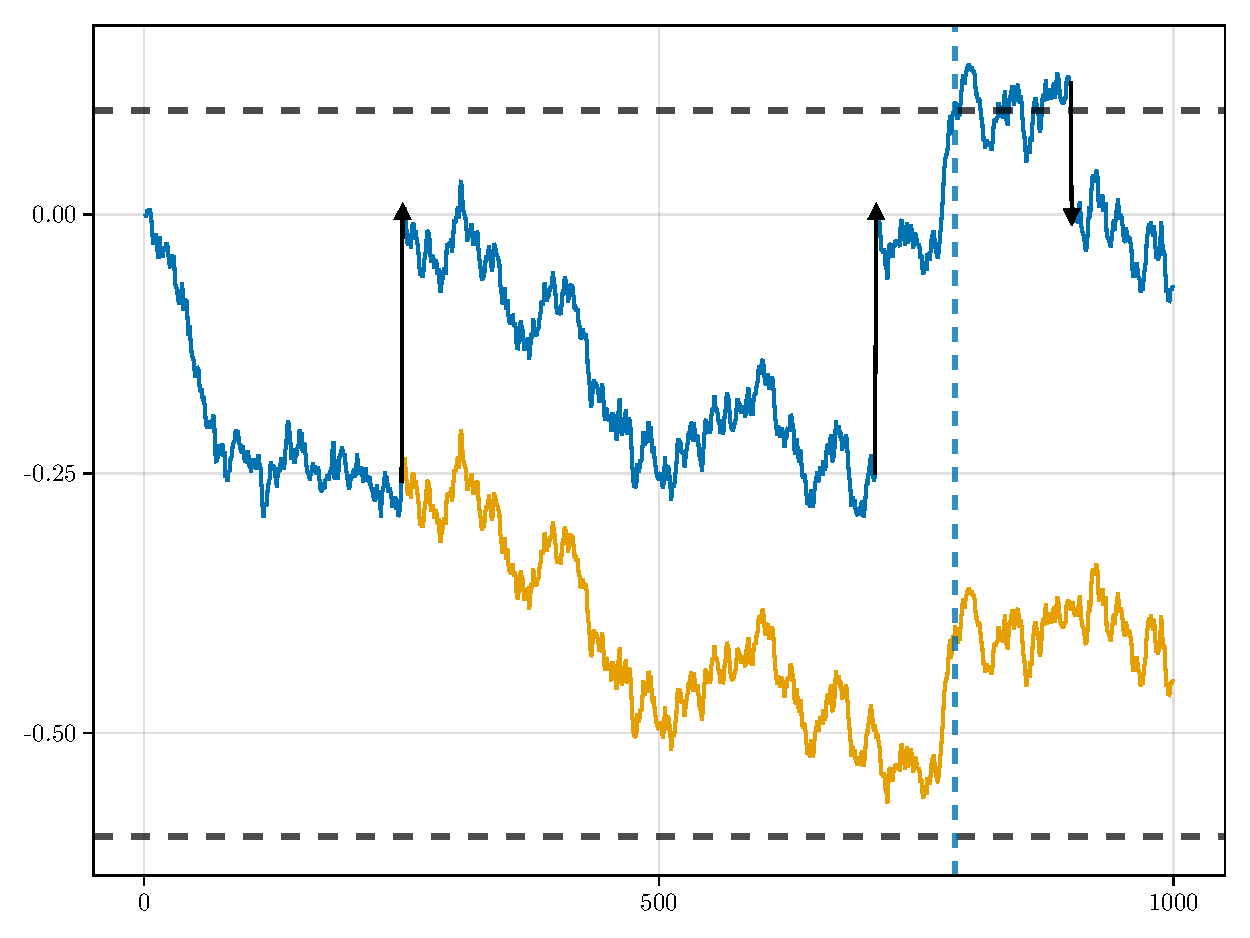
\includegraphics[width=0.9\textwidth]{wiener-sim/tr-resetting.pdf}
\end{frame}



\begin{frame}
\frametitle{Resetowanie Stochastyczne - ogólniej}
Załóżmy, że mamy pewną zmienną losową $T:\Omega \to [0, \infty)$, która ma interpretację jak FPT. \\~\\
\pause
Niech $R:\Omega \to [0, \infty)$ będzie niezależne od $T$ i ma interpretację czasu po jakim resetujemy.
\pause
\begin{block}{Definicja}
Zdefiniujmy\footnotemark{} $T_R$ ("$T$ \emph{pod wpływem resetowania}") jako
\begin{equation}
T_R = \begin{cases}
T &,~\text{gdy}~ T < R \\
R + T_R' &,~\text{gdy}~ T \ge R~,
\end{cases}
\end{equation}
gdzie $T_R'$ jest niezależne od $T_R$ i ma identyczny rozkład.
\end{block}

\footnotetext{Bardziej formalnie można użyć ciągów i.i.d. zmiennych losowych \\ o rozkładach jak rozkłady $T$ i $R$.}
\end{frame}

\begin{frame}
\frametitle{Resetowanie Stochastyczne - przykład optymalizacji MFPT}
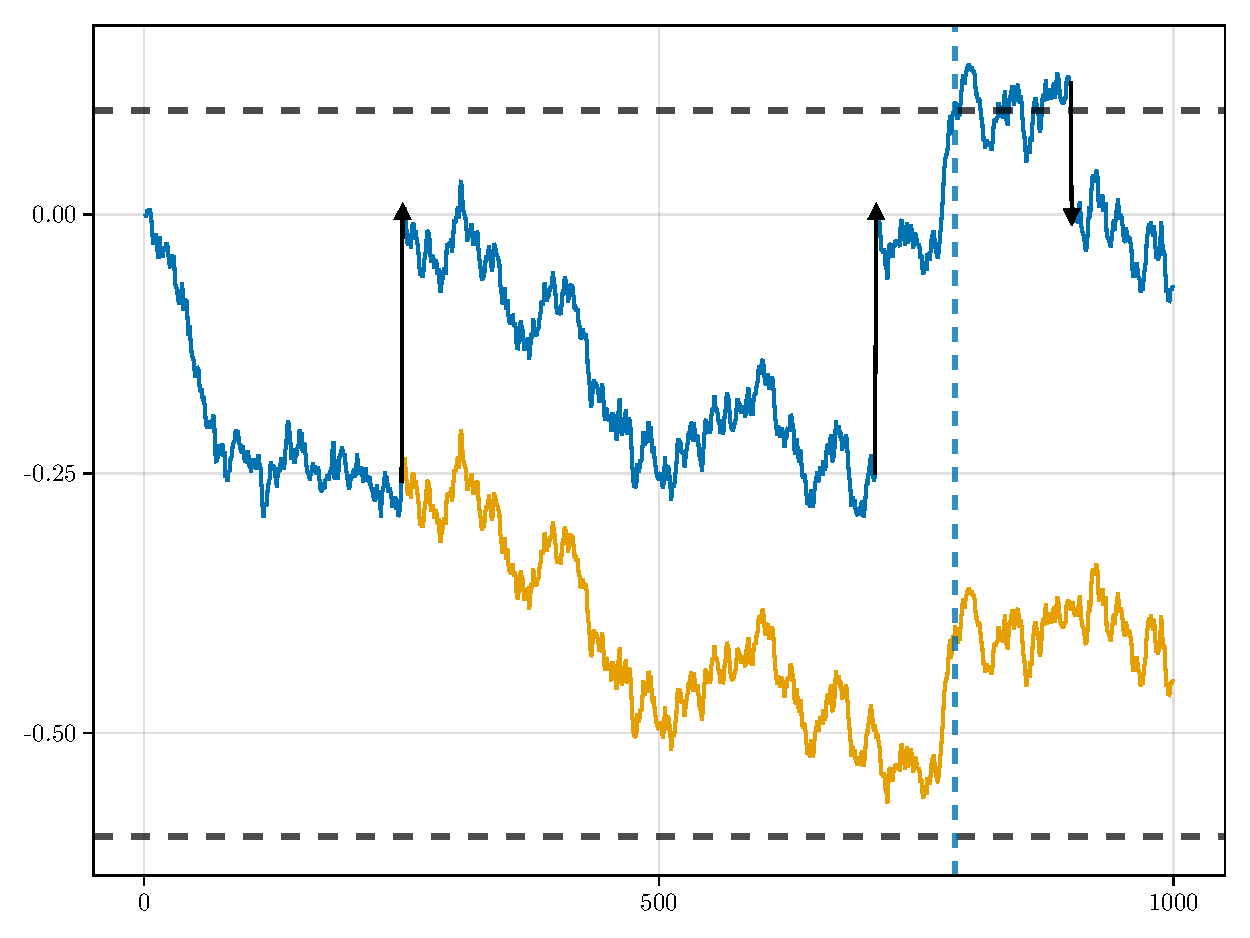
\includegraphics[width=0.9\textwidth]{wiener-sim/tr-resetting.pdf}
\end{frame}


\begin{frame}
\frametitle{Ile można powiedzieć na podstawie przyjętego modelu?}
Znajdźmy wyrażenie na MFPT przy założeniu resetowania
\begin{equation}
\T_R = \E T_R = \E [T ; T < R] + \E [R + T_R' ; T \ge  R]
\end{equation}
\pause
Wiemy, że $T_R'$ nie zależy od $T, R$ i ma ten sam rozkład co $T_R$
\begin{equation}
\T_R = \E [T ; T < R] + \E [R; T \ge  R] + \T_R \p( T \ge  R)
\end{equation}
\pause
Po dalszych przekształceniach
\begin{equation}
\boxed{   \T_R = \frac{\E \min{(T, R)}}{\p(T < R)}   }
\end{equation}
\end{frame}

\begin{frame}
\frametitle{Resetowanie Poissonowskie}
Załóżmy, że $R \sim \rm{Exp}(r)$, czyli $f_R(t) = r e^{-rt} \cdot \chi_{[0, \infty)}(t)$.\\~\\
Jeśli tak jest, to mówimy że resetowanie jest Poissonowskie i parametr $r$~nazywamy szybkością resetowania (ang. reset rate).\\~\\
\pause
Wówczas transformata Laplace'a $\Lap{T_R}(s) \equiv \E e^{-sT_R}$ zmiennej $T_R$ ma postać\footnotemark{}
\begin{equation}
\Lap{T_R}(s) = \frac{\Lap{T}(r+s)} {\frac{s}{s+r} + \frac{r}{s+r} \Lap{T}(r+s)}
\end{equation}

\vfill
Zauważmy, że $\lim_{s \to 0} \Lap{T_R}(s) = 1$ i zbadajmy momenty $T_R$.

\footnotetext{A. Pal and S. Reuveni, Phys. Rev. Lett. 118, 030603 (2017)}
\end{frame}


\begin{frame}
\frametitle{Resetowanie Poissonowskie}
\begin{equation}
\T_R = \E T_R = - \frac{d}{ds} \Lap{T_R}(s) \Big |_{s = 0} =  \frac{1}{r} \left ( \frac{1}{\Lap{T}(r)} - 1 \right )
\end{equation}
\pause
Załóżmy, że dla dostatecznie małych $r$ funkcję $\Lap{T}(r)$ możemy aproksymować wielomianem\footnotemark{} od zmiennej $r$
\begin{equation}
\Lap{T}(r) = 1 - m_1 r + \frac{1}{2} m_2 r^2 + o(r^2),
\end{equation}
gdzie $m_1 = \E [T]$ i $m_2 = \E [X^2]$ z własności transformaty Laplace'a (związek z funkcją tworzącą).
\pause
Wówczas
\begin{equation}
\T_R = \T +  \left ( \T^2 -  \frac{1}{2} \E [T^2] \right ) r + o(r^2)~.
\end{equation}

\footnotetext{Zakładamy, że $\Lap{T}$ jest klasy $\mathcal{C}^2$ na pewnym otoczeniu 0}
\end{frame}

\section{Współczynnik Zmienności CV - (ang. Coefficient of Variation)}

\begin{frame}
\frametitle{Warunek bazujący na CV (ang. Coefficient of Variation)}
\begin{equation}
\T_R = \T + \frac{1}{2} \left ( \T^2 - \E [(T - \T)^2] \right ) r + o(r^2)
\end{equation}
daje nam warunek wystarczający, aby wprowadzenie resetowania zmniejszało MFPT.
\pause
\begin{block}{Wniosek (Twierdzenie)}
Jeśli $T$ ma interpretację jak FPT i $CV(T) > 1$, to istnieje $r$ (małe) tże.: 
\begin{equation}
\boxed{ \T_R < \T, \quad \text{dla}~ R \sim \rm{Exp}(r) }.
\end{equation}
W założeniach $CV(T)$ oznacza współczynnik zmienności 
\begin{equation}
CV(T) = \frac{\sigma(T)}{\E [T]} = \frac{\sqrt{ \E [(T - \T)^2] }}{\T} = \sqrt{\frac{\E [T^2]}{\T^2} - 1}
\end{equation}
\end{block}

\end{frame}

\begin{frame}
\frametitle{Warunek bazujący na CV}
\begin{block}{Wniosek (Twierdzenie)}
Jeśli $T$ ma interpretację jak FPT i $CV(T) > 1$, to istnieje $r$ (małe) tże.: 
\begin{equation}
\boxed{ \T_R < \T, \quad \text{dla}~ R \sim \rm{Exp}(r) }.
\end{equation}
W założeniach $CV(T)$ oznacza współczynnik zmienności 
\begin{equation}
CV(T) = \frac{\sigma(T)}{\E [T]} = \frac{\sqrt{ \E [(T - \T)^2] }}{\T} = \sqrt{\frac{\E [T^2]}{\T^2} - 1}
\end{equation}
\end{block}

Ważne: {\color{magenta}
Wystarczy zbadać własności procesu (ucieczek) bez resetowania, żeby powiedzieć coś o resetowaniu.
}
\end{frame}

\begin{frame}
\frametitle{Zastosowanie dla  procesu Wienera}
\begin{columns}
\column{0.5\textwidth}
\begin{figure}
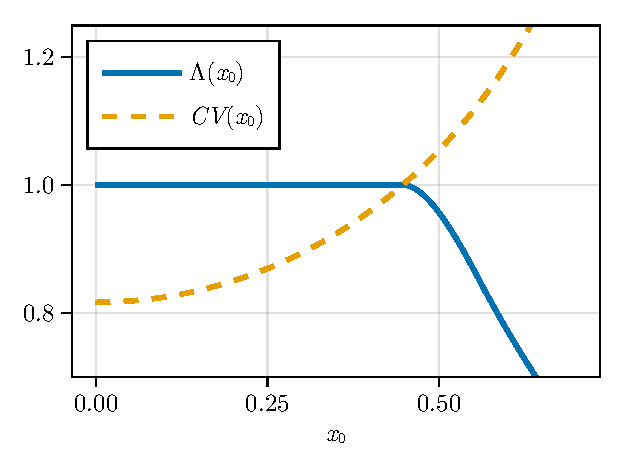
\includegraphics[width=\textwidth]{wiener-sim/CV-MFPT.pdf}
\caption{Znormalizowane MFPT dla procesu Wienera startującego w $x_0$ i uciekającego z przedziału $(-1, 1)$.}
\end{figure}

\column{0.5\textwidth}
Aby zobaczyć kiedy resetowanie pomaga (i jak się ma do $CV$) definiujemy
\begin{equation}
\Lambda(x_0) = \frac{\min_{r \ge 0}{(\T_R)}}{\T},
\end{equation}
czyli minimalne $\T_R$ (dla resetowania Poissonowskiego) znormalizowane przez $\T$.\\
Ponadto MFPT dla ucieczki z $(-L, L)$ kiedy proces startuje w $x_0$ wynosi
\begin{equation}
\T(x_0) = \frac{L^2 - x^2_0}{2}
\end{equation}
\end{columns}

\end{frame}


\begin{frame}
\frametitle{Bibliografia}
\end{frame}

\end{document}
